\documentclass[11pt,a4paper]{article}
\usepackage[utf8]{inputenc}
\usepackage{lmodern}
\usepackage[T1]{fontenc}
\usepackage[finnish]{babel}
\usepackage{graphicx}
\usepackage{epstopdf}
\usepackage{listings} 
\usepackage{xcolor}
\usepackage{textcomp}

\definecolor{dkgreen}{rgb}{0,0.6,0}
\definecolor{gray}{rgb}{0.5,0.5,0.5}
\definecolor{amber}{rgb}{1.0, 0.49, 0.0}

%Java lstset
\lstset{frame=none,
  language=Java,
  aboveskip=3mm,
  belowskip=3mm,
  showstringspaces=false,
  columns=flexible,
  basicstyle={\small\ttfamily},
  numbers=none,
  numberstyle=\tiny\color{gray},
  keywordstyle=\color{blue},
  commentstyle=\color{dkgreen},
  stringstyle=\color{amber},
  breaklines=true,
  breakatwhitespace=true,
  tabsize=3
}

%Multi-byte encoding
\lstset{literate=
  {á}{{\'a}}1 {é}{{\'e}}1 {í}{{\'i}}1 {ó}{{\'o}}1 {ú}{{\'u}}1
  {Á}{{\'A}}1 {É}{{\'E}}1 {Í}{{\'I}}1 {Ó}{{\'O}}1 {Ú}{{\'U}}1
  {à}{{\`a}}1 {è}{{\`e}}1 {ì}{{\`i}}1 {ò}{{\`o}}1 {ù}{{\`u}}1
  {À}{{\`A}}1 {È}{{\'E}}1 {Ì}{{\`I}}1 {Ò}{{\`O}}1 {Ù}{{\`U}}1
  {ä}{{\"a}}1 {ë}{{\"e}}1 {ï}{{\"i}}1 {ö}{{\"o}}1 {ü}{{\"u}}1
  {Ä}{{\"A}}1 {Ë}{{\"E}}1 {Ï}{{\"I}}1 {Ö}{{\"O}}1 {Ü}{{\"U}}1
  {â}{{\^a}}1 {ê}{{\^e}}1 {î}{{\^i}}1 {ô}{{\^o}}1 {û}{{\^u}}1
  {Â}{{\^A}}1 {Ê}{{\^E}}1 {Î}{{\^I}}1 {Ô}{{\^O}}1 {Û}{{\^U}}1
  {Ã}{{\~A}}1 {ã}{{\~a}}1 {Õ}{{\~O}}1 {õ}{{\~o}}1
  {œ}{{\oe}}1 {Œ}{{\OE}}1 {æ}{{\ae}}1 {Æ}{{\AE}}1 {ß}{{\ss}}1
  {ű}{{\H{u}}}1 {Ű}{{\H{U}}}1 {ő}{{\H{o}}}1 {Ő}{{\H{O}}}1
  {ç}{{\c c}}1 {Ç}{{\c C}}1 {ø}{{\o}}1 {å}{{\r a}}1 {Å}{{\r A}}1
  {€}{{\euro}}1 {£}{{\pounds}}1 {«}{{\guillemotleft}}1
  {»}{{\guillemotright}}1 {ñ}{{\~n}}1 {Ñ}{{\~N}}1 {¿}{{?`}}1
}


\begin{document}
\author{Ville Manninen
\thanks{mooc.fi: vw.manninen@gmail.com}
\thanks{opiskelijanumero: 014922187}}
\date{\today}
\title{Tietokantojen perusteet, kevät 2020 \\
Harjoitustyön raportti}
\maketitle
\begin{center}
\vspace{2cm}

\includegraphics{university-of-helsinki-2.eps} 
\end{center}
\newpage
\tableofcontents
\newpage
\section{Esittely}

\subsection{Tavoite}
Harjoitustyön tavoitteena on luoda esimerkkisovellus tietokannan käytöstä sovelluksessa.
Harjoitustyön sovelluksen ohjelmointi on toteutettu Java kielellä käyttäen NetBeans kehitysympäristöä. Ohjelman tietokantaa pitää yllä SQLite ja sitä tukeva ajuri.

\subsection{Ohjelman ominaisuudet}
Ohjelmalla on seuraavat ominaisuudet.
\begin{itemize}
\item Tietokannan luominen kun tietokanta puuttuu tai on puutteellinen.
\item Asiakkaiden lisääminen tietokantaan.
\item Paikkojen lisäämien tietokantaan.
\item Pakettien lisääminen tietokantaan.
\item Tapahtumien lisääminen tietokantaan.
\item Pakettien tapahtumien hakeminen.
\item Asiakkaan pakettien hakeminen ja yksittäisten pakettien tapahtumien lukumäärä.
\item Tapahtumien määrän hakeminen halutusta paikasta päivämäärällä.
\item Tehokkuustestin suorittaminen.
\end{itemize}
\newpage
\subsection{Komentorivi komennot}
Ohjelmalle voidaan antaa komentoja syöttmällä komentoa kuvaava numero komentoriville. Ohjelmalla on seuraavat, numeroidut komennot.
\begin{description}
\item \textbf{1} lisää uuden asiakkaan tietokantaan.
\item \textbf{2} lisää uuden paikan tietokantaan.
\item \textbf{3} lisää uuden paketin tietokantaan.
\item \textbf{4} lisää uuden tapahtuman tietokantaan.
\item \textbf{5} tulostaa paketin tapahtumat tietokannasta.
\item \textbf{6} tulostaa asiakkaan paketit ja niihin liittyvien tapahtumien määrän tietokannasta.
\item \textbf{7} tulostaa tapahtumien määrän haku paikasta tietyllä päivämäärällä tietokannasta.
\item \textbf{8} suorittaa tehokkuustestin ja tulostaa testin tulokset käyttäjälle.
\item \textbf{9} luo tietokannan.
\item \textbf{0} Sulkee ohjelman.
\end{description}

\newpage
\section{Kaaviot ja Skeemat}
\subsection{Tietokantakaavio}
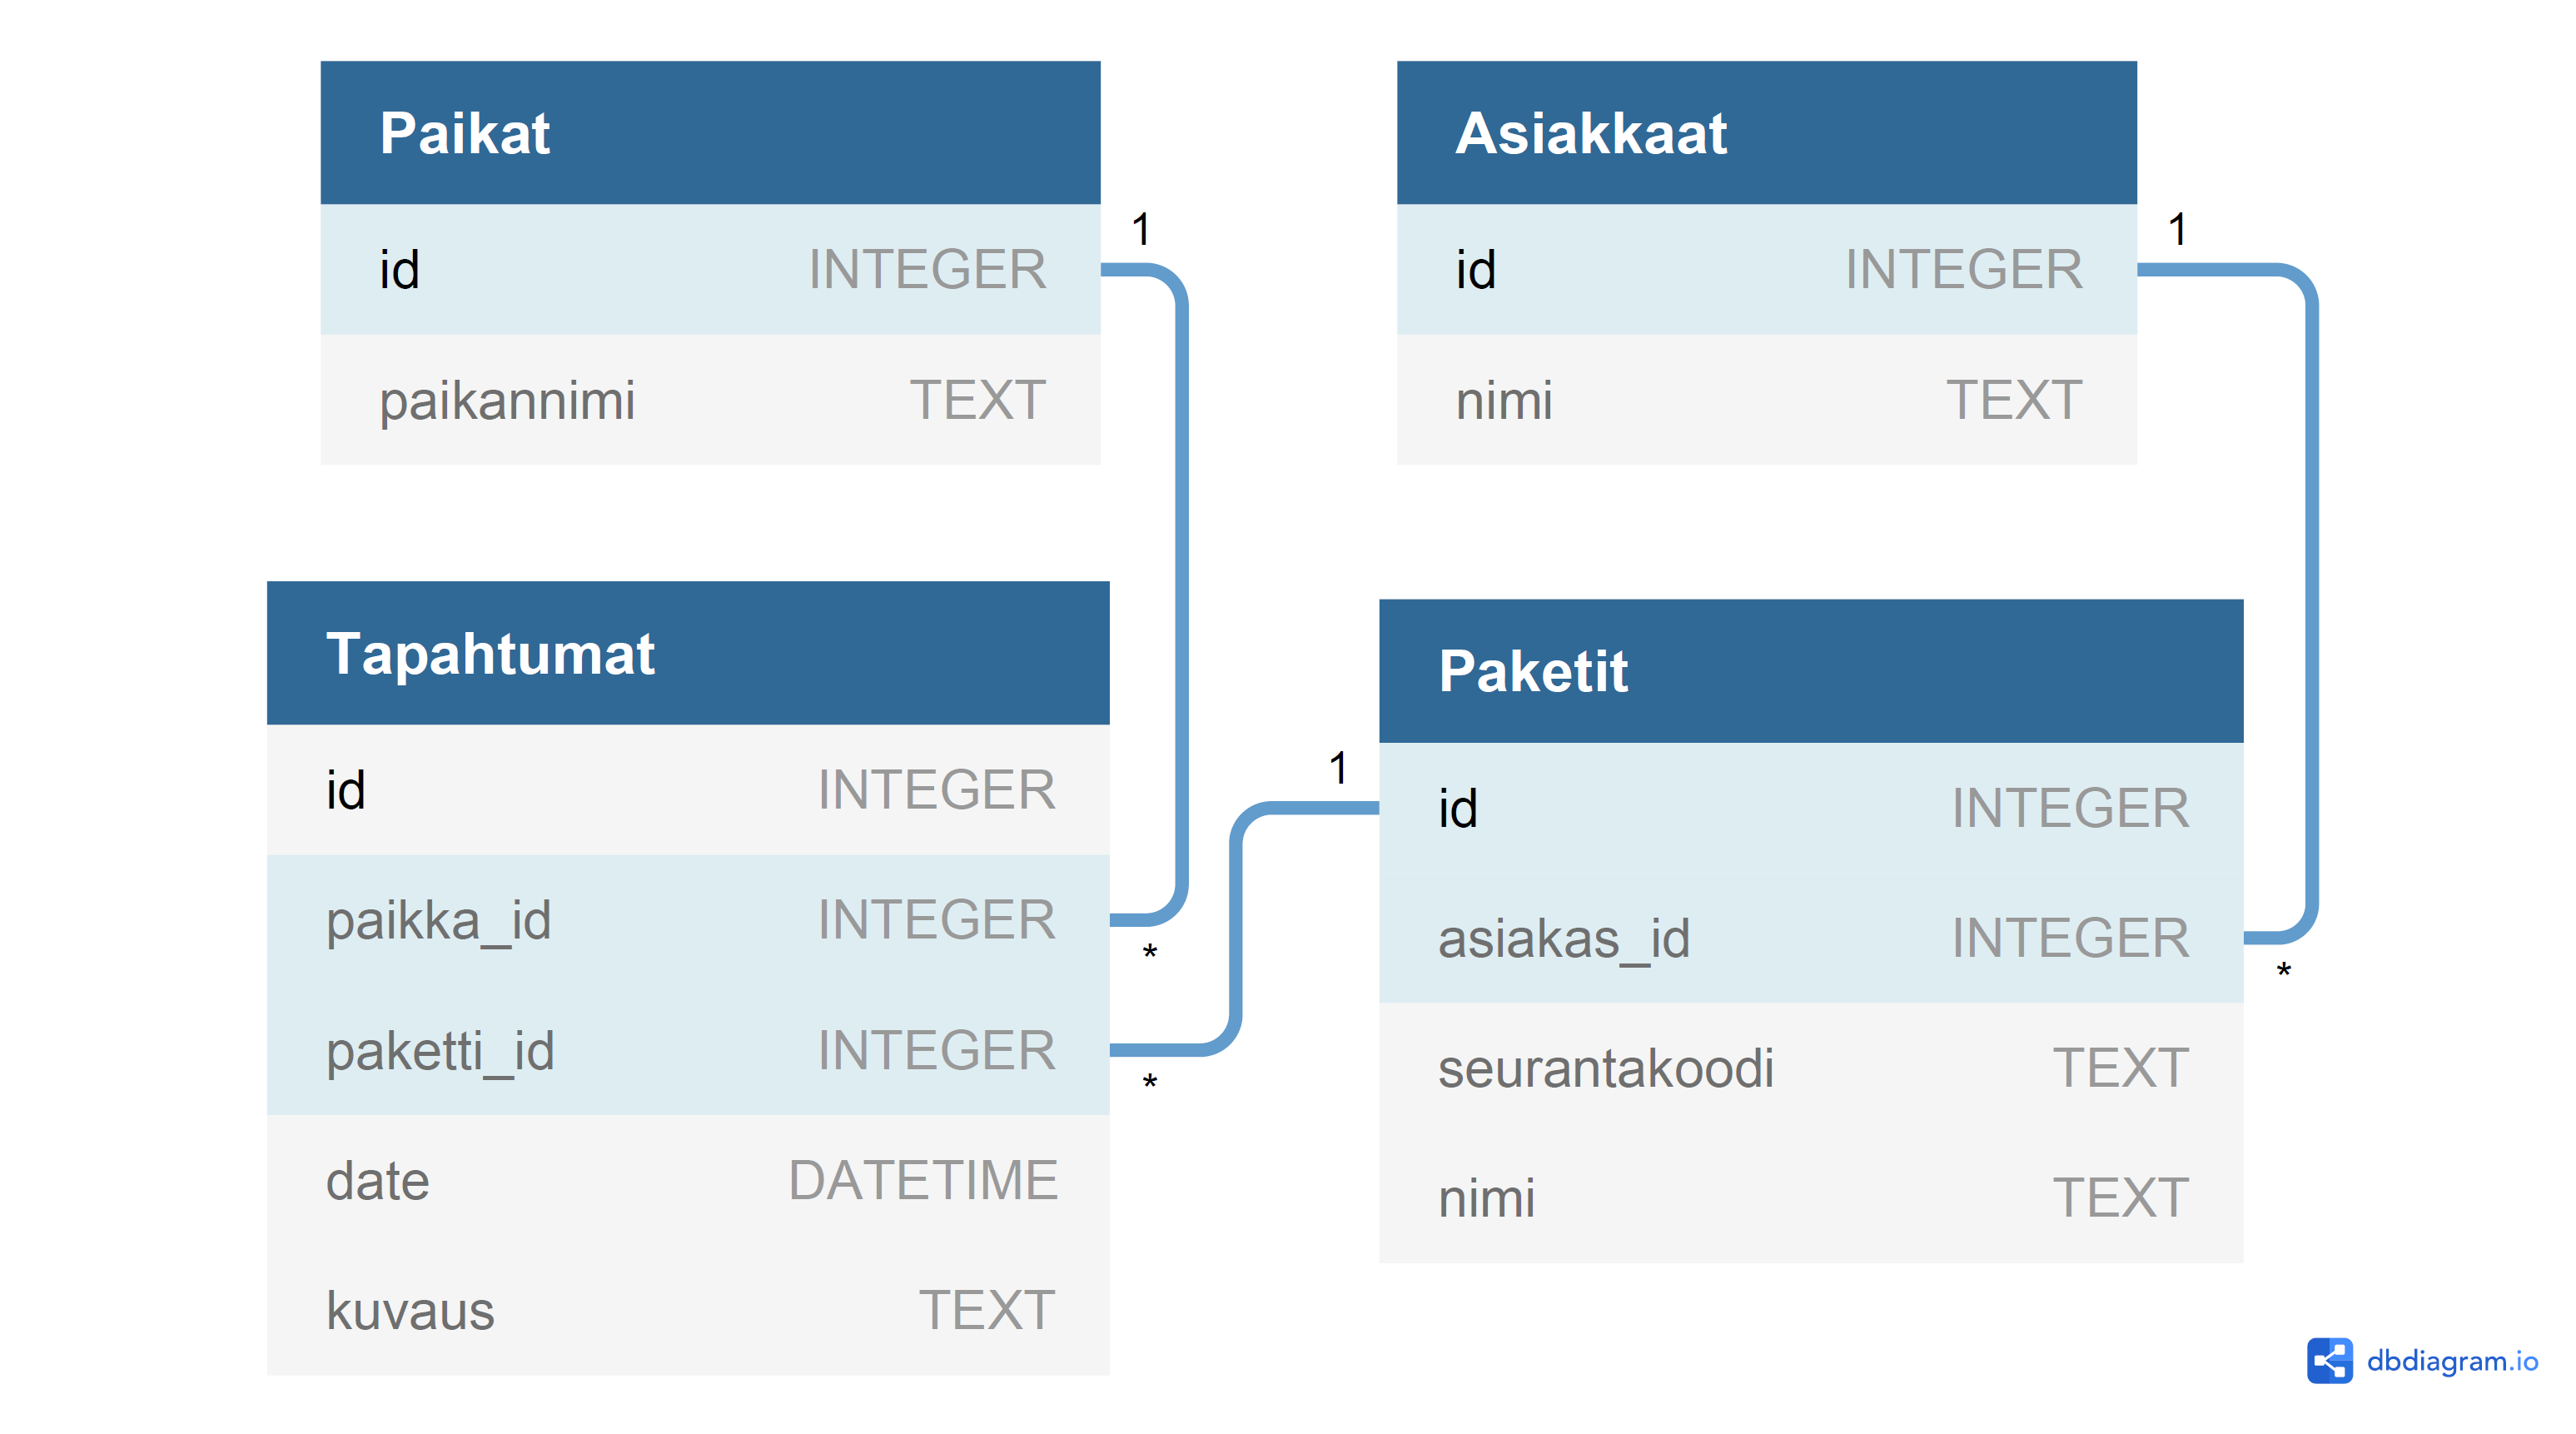
\includegraphics[scale=0.25]{tietokanta_kaavio.png} 

\subsection{SQL-skeema}
\lstset{frame=none,
  language=SQL,
  aboveskip=3mm,
  belowskip=3mm,
  showstringspaces=false,
  columns=flexible,
  basicstyle={\small\ttfamily},
  numbers=none,
  numberstyle=\tiny\color{gray},
  keywordstyle=\color{blue},
  commentstyle=\color{dkgreen},
  stringstyle=\color{amber},
  breaklines=true,
  breakatwhitespace=true,
  tabsize=3
}
\begin{lstlisting}

CREATE TABLE Asiakkaat (id INTEGER PRIMARY KEY, nimi TEXT NOT NULL UNIQUE);

CREATE TABLE Paikat (id INTEGER PRIMARY KEY, paikannimi TEXT NOT NULL UNIQUE);

CREATE TABLE Paketit (id INTEGER PRIMARY KEY, asiakas_id INTEGER NOT NULL, seurantakoodi TEXT NOT NULL UNIQUE);

CREATE TABLE Tapahtumat (id INTEGER PRIMARY KEY, paikka_id INTEGER NOT NULL, paketti_id INTEGER NOT NULL, date DATETIME NOT NULL, kuvaus TEXT NOT NULL);
\end{lstlisting}
\newpage

\section{Tehokkuustesti}

\subsection{Testin vaiheet}
Ohjelmalla voidaan suorittaa tehokkuustesti jonka avulla voidaan testata tietokannan tehokkuutta. Tehokkuustesti suorittaa ennalta määriteltyjä muutoksia tietokantaan ja tulostaa testeihin käytetyn ajan. Tehokkuustesti luo uuden tietokannan johon testin aikana luodut arvot tallennetaan, testin jälkeen ohjelma palaa käyttämään vanhaa tietokantaa.

Testi koostuu kuudesta eri vaiheesta, testin vaiheissa yhdestä neljään tietokantaan lisätään tuhat asiakasta, paikkaa ja pakettia. Seuraavaksi tietokantaan lisätään miljoona tapahtumaa käyttäen satunnaisesti tietokantaan lisättyjä arvoja. Ohjelmaa testatessa tuhannen arvon lisääminen tapahtui alle sekunnin kymmenesosassa kun taas miljoonaa arvoa lisätessä aikaa kului 10-12 sekunttia, tästä nähdään että ohjelman tehokkuuteen vaikuttaa merkittävästi tietokantaan lisättävien arvojen määrä.

Viimeisissä vaiheissa viisi ja kuusi testi suorittaa kyselyitä joissa haetaan tuhannen asiakkaan pakettien määrä, sekä tuhannen paketin tapahtumien määrä. Mainituissa vaiheissa testin tehokkuuteen vaikutti eniten indeksien käyttö.

\subsection{Ilman indeksiä}
Ilman lisättyä indeksiä pakettien hakemiseen tietokannasta aikaa kului alle sekunnin, mutta tapahtumia haettaessa aikaa kuluikin yli minuutin. Tarkastelun jälkeen huomataan että tapahtumaa haettaessa SQLite suorittaa alikyselyn jokaisen tapahtuman kohdalla. Mainittu alikysely etsii paketit taulukosta nimellä haluttua pakettia, tämä käsittely hidastaa kyselyä merkittävästi.

\subsection{Indeksin lisäämisen jälkeen}
Tehokkuuden lisäämiseksi voidaan paketin arvolle nimi luoda hakemistorakenne paketin nimelle. Käyttämällä SQLiten CREATE INDEX toimintoa, indeksin lisäämisen jälkeen tapahtuma kysely hakee nimellä paketin id-numeron tehokkaasti. Indeksin lisäämisen jälkeen tapahtuma kysely vei aikaa noin sekunnin.

\newpage
\section{Tietokannan eheys}
Ohjelman tietokannan eheyttä pidetään yllä käyttämällä SQLiten sekä Javan tarjoamia ominaisuuksia. Tietokantaan ei ole mahdollista luoda samannimisiä asiakkaita tai paikkoja, eikä tietokantaan luoduille paketeille saa antaa samaa seurantakoodia.

Samannimisiä syötteitä valvotaan SQLiten rajoitteella UNIQUE, joka varmistaa ettei samaan tauluun lisätä samannimisiä arvoja. Lisäksi SQLiten rajoitteella NOT NULL valvotaan että sarakkeisiin ei lisätä tyhjiä arvoja, tätä käytetään hyväksi esimerkiksi kun lisätään arvoja jotka viittaavat muihin sarakkeisiin, alikysely palauttaa arvon NULL jos arvoa johon viitataan ei löydy tietokannasta.
 
Ohjelma tarkistaa käyttäjän antamat syötteet ja hylkää syötteet jotka eivät kelpaa ohjelmalle. Tietokantaan lisättäessä paketteja tai tapahtumia jotka viittaavat toiseen taulukkoon tallennettuun tietoon, sovellus varmistaa että viitatut tiedot löytyvät tietokannassa.

Tapauksissa joissa ohjelmalle syötetään arvo jota se ei kelpuuta ohjelma tulostaa käyttäjälle virheilmoituksen ja jatkaa ohjelman suorittamista. Virheilmoitukset kertovat käyttäjälle miksi annettu syöte ei kelvannut. Tapauksissa joissa SQLite antaa virheilmoituksen tulostetaan myös tämä käyttäjälle. 

\newpage
\section{Lähdekoodi}

\subsection*{Esittely}
Seuraavasta kappaleesta löytyy ohjelman lähdekoodi, sekä lyhyt esittely ohjelman rakenteesta:

Ohjelma koostuu kuudesta luokasta, luokka Main suorittaa komentorivisovellusta, kun tehdään muutoksia tietokantaan kutsutaan luokkaa DatabaseManager. DatabaseManager luokka luo ja muokkaa tietokanna taulukoita joista jokaisella on oma luokkansa. Ohjelman lähdekoodi ja raportti löytyvät myös alla olevasta osoitteesta.

\begin{center}
\textbf{https://github.com/Viltska/sql-app-training}
\end{center}
\newpage

\subsection*{Main.java}
\lstinputlisting[language=Java]{E:/Koulu/Tietokantojen Perusteet/sql-app-training/src/Main.java}
\newpage

\subsection*{DatabaseManager.java}
\lstinputlisting[language=Java]{E:/Koulu/Tietokantojen Perusteet/sql-app-training/src/DatabaseManager.java}
\newpage

\subsection*{Asiakkaat.java}
\lstinputlisting[language=Java]{E:/Koulu/Tietokantojen Perusteet/sql-app-training/src/Asiakkaat.java}
\newpage

\subsection*{Paikat.java}
\lstinputlisting[language=Java]{E:/Koulu/Tietokantojen Perusteet/sql-app-training/src/Paikat.java}
\newpage

\subsection*{Paketit.java}
\lstinputlisting[language=Java]{E:/Koulu/Tietokantojen Perusteet/sql-app-training/src/Paketit.java}
\newpage

\subsection*{Tapahtumat.java}
\lstinputlisting[language=Java]{E:/Koulu/Tietokantojen Perusteet/sql-app-training/src/Tapahtumat.java}
\end{document}